
%(BEGIN_QUESTION)
% Copyright 2006, Tony R. Kuphaldt, released under the Creative Commons Attribution License (v 1.0)
% This means you may do almost anything with this work of mine, so long as you give me proper credit

Calculate the 0\%, 50\%, and 100\% calibration points for the $\Delta$P transmitter to measure liquid level in this vessel, given a range of 0 to 30 feet and a specific gravity of 0.85.  Note that the ``low'' side of the transmitter connects to the top of the vessel to compensate for vapor pressure inside the vessel.  This tube is called a ``dry leg'' because there is no liquid inside of it:

$$\includegraphics[width=15.5cm]{i00262x01.eps}$$

% No blank lines allowed between lines of an \halign structure!
% I use comments (%) instead, so that TeX doesn't choke.

$$\vbox{\offinterlineskip
\halign{\strut
\vrule \quad\hfil # \ \hfil & 
\vrule \quad\hfil # \ \hfil & 
\vrule \quad\hfil # \ \hfil \vrule \cr
\noalign{\hrule}
%
% First row
\% of span & $\Delta$P ("H$_{2}$O) & Output (mA) \cr
%
\noalign{\hrule}
%
% Another row
0 &  &  \cr
%
\noalign{\hrule}
%
% Another row
50 &  &  \cr
%
\noalign{\hrule}
%
% Another row
100 &  &  \cr
%
\noalign{\hrule}
} % End of \halign 
}$$ % End of \vbox

Now suppose the vessel is heated, and the liquid inside the vessel emits condensible vapors.  These vapors will condense inside low-side tube leading to the $\Delta$P transmitter which is cooler than the storage vessel, resulting in a ``wet leg'' instead of a ``dry leg.''  In other words, the transmitter will now ``see'' a constant column of liquid (SG = 0.85) 30 feet high connected to its ``low'' process port:

$$\includegraphics[width=15.5cm]{i00262x02.eps}$$

Re-calculate the 0\%, 50\%, and 100\% calibration points for the $\Delta$P transmitter to measure liquid level in this vessel with a wet reference leg instead of a dry reference leg.

% No blank lines allowed between lines of an \halign structure!
% I use comments (%) instead, so that TeX doesn't choke.

$$\vbox{\offinterlineskip
\halign{\strut
\vrule \quad\hfil # \ \hfil & 
\vrule \quad\hfil # \ \hfil & 
\vrule \quad\hfil # \ \hfil \vrule \cr
\noalign{\hrule}
%
% First row
\% of span & $\Delta$P ("H$_{2}$O) & Output (mA) \cr
%
\noalign{\hrule}
%
% Another row
0 &  &  \cr
%
\noalign{\hrule}
%
% Another row
50 &  &  \cr
%
\noalign{\hrule}
%
% Another row
100 &  &  \cr
%
\noalign{\hrule}
} % End of \halign 
}$$ % End of \vbox

\underbar{file i00262}
%(END_QUESTION)





%(BEGIN_ANSWER)

{\bf Dry leg:}

% No blank lines allowed between lines of an \halign structure!
% I use comments (%) instead, so that TeX doesn't choke.

$$\vbox{\offinterlineskip
\halign{\strut
\vrule \quad\hfil # \ \hfil & 
\vrule \quad\hfil # \ \hfil & 
\vrule \quad\hfil # \ \hfil \vrule \cr
\noalign{\hrule}
%
% First row
\% of span & $\Delta$P ("H$_{2}$O) & Output (mA) \cr
%
\noalign{\hrule}
%
% Another row
0 & 0 & 10 \cr
%
\noalign{\hrule}
%
% Another row
50 & 153 & 30 \cr
%
\noalign{\hrule}
%
% Another row
100 & 306 & 50 \cr
%
\noalign{\hrule}
} % End of \halign 
}$$ % End of \vbox

\vskip 10pt

{\bf Wet leg:}

% No blank lines allowed between lines of an \halign structure!
% I use comments (%) instead, so that TeX doesn't choke.

$$\vbox{\offinterlineskip
\halign{\strut
\vrule \quad\hfil # \ \hfil & 
\vrule \quad\hfil # \ \hfil & 
\vrule \quad\hfil # \ \hfil \vrule \cr
\noalign{\hrule}
%
% First row
\% of span & $\Delta$P ("H$_{2}$O) & Output (mA) \cr
%
\noalign{\hrule}
%
% Another row
0 & -306 & 10 \cr
%
\noalign{\hrule}
%
% Another row
50 & -153 & 30 \cr
%
\noalign{\hrule}
%
% Another row
100 & 0 & 50 \cr
%
\noalign{\hrule}
} % End of \halign 
}$$ % End of \vbox




%(END_ANSWER)





%(BEGIN_NOTES)


%INDEX% Measurement, level: hydrostatic pressure (elevated zero)
%INDEX% Measurement, level: hydrostatic pressure (``wet'' reference leg)

%(END_NOTES)


